\documentclass[11pt]{article}
\usepackage{amsfonts}
\usepackage{amsmath}
\usepackage{amsthm}
\usepackage{amssymb}
\usepackage{mathrsfs}
\usepackage[fit]{truncate}
\usepackage{acl2012}
\usepackage{times}
\usepackage{latexsym}
\usepackage{amsmath}
\usepackage{url}
\usepackage{graphicx}
\usepackage{caption}
\usepackage{multirow}
\usepackage{dblfloatfix}
\usepackage{float}
\usepackage{subfigure}
\DeclareMathOperator*{\argmax}{arg\,max}
\setlength\titlebox{5.2cm}    % Expanding the titlebox



\newcommand{\affliationPenn}{\ensuremath{{}^\text{1}}}
\newcommand{\affliationJHU}{\ensuremath{{}^\text{2}}}

\title{A large scale study of the languages spoken (by bilinguals) on Mechanical Turk}
\title{The Language Demographics of  Amazon Mechanical Turk}

\author{Ellie Pavlick\affliationPenn \ \ \ \ \ \ \ \ \ \ Dmitry Kachaev\affliationJHU \ \ \ \ \ \ \ \ \ \  Chris Callison-Burch\affliationPenn$^{,}$\affliationJHU \\
\affliationPenn Computer and Information Science Department, University of Pennsylvania \\
\affliationJHU Human Language Technology Center of Excellence, Johns Hopkins University \\
  }
  
% Anonymized for submission
\author{}

\date{}

\begin{document}
\maketitle

\begin{abstract}
We present a large scale study of the languages spoken by bilingual workers on Mechanical Turk (MTurk).  
We establish a  methodology for determining the language skills of anonymous crowd workers that is more robust than simple surveying.  We validate workers' self-reported language skill claims by measuring their ability to correctly translate words, and by geolocating workers to see if they reside in countries where the languages are likely to be spoken. Rather than posting a one-off survey, we posted paid tasks consisting of 1,000 assignments to translate a total of 10,000 words in each of 119 languages.  Our study ran for several weeks, and was highly visible on the MTurk crowdsourcing platform, increasing the chances that bilingual workers would complete it.  Our study was useful both to create bilingual dictionaries and to act as census of the bilingual speakers on MTurk.  We use this data to recommend languages with the largest speaker populations as good candidates for other researchers who want to  develop crowdsourced, multilingual technologies.

\end{abstract}

\section{Overview}
Crowdsourcing is a promising new mechanism for collecting data for natural language processing research. Access to a fast, cheap, and flexible workforce allows us to collect new types of data, potentially enabling new language technologies.
Because crowdsourcing platforms like Amazon Mechanical Turk (MTurk) give researchers access to a worldwide workforce, one obvious application of crowdsourcing is the creation of multilingual technologies. 
With an increasing number of active crowd workers located outside of the United States, there is even the potential to reach fluent speakers of lower resource languages.
In this paper, we investigate the feasibility of hiring language informants on MTurk by conducting the first large-scale demographic study of the languages spoken by workers on the platform. 

%Access to a fast, cheap, and flexible workforce has changed the way we collect data, and holds promise for enabling future language technologies. Crowdsourced work has proven effective for collecting massive amounts of simple data annotations, such as annotating data for face recognition software and labeling sentiment in twitter data. As the demands and expectations of automated systems progress, and the complexity of the data required for training increases, however, it becomes natural to ask about the strengths and limitations of the crowd as annotators for natural language data.
%We evaluate the language skills of bilingual workers on Amazon's Mechanical Turk, and their ability to provide translated data for statistical machine translation. Collecting parallel translated texts has traditionally been assumed to require a higher level of expertise than what is available from non-professional crowd workers. However, with an increasing number of active crowd workers located outside of the United States, the potential to access fluent speakers of lower resource languages makes crowdsourcing an attractive resource for translation.

There are several complicating factors when trying to take a census of workers on MTurk.  The workers' identities are anonymized, and Amazon provides no information about their countries of origin or their language abilities.  Posting a simple survey to have workers self-report this information may be inadequate, since (a) many worker may never see the survey, (b) many opt not to do one-off surveys since potential payment is low, and (c) validating the answers of respondents is not straightforward. 

Our study establishes a methodology for determining the language demographics of anonymous crowd workers that is more robust than simple surveying. We ask workers what languages they speak and what country they live in, and validate their claims by measuring their ability to correctly translate words and by geolocating them.  To increase the visibility and the desirability of our tasks, we post 1,000 assignments in each of 119 languages.  These tasks each consist of translating 10 foreign words into English.  Two of the 10 words have known translations, allowing us to validate the the workers' translations are accurate.  We construct bilingual dictionaries with up to 10,000 entries, with the majority of entries being new. 

Surveying thousands of workers allows us to analyze current speaker populations for more than 100 languages.  The data also allows us to answer questions like: 
How quickly is work completed in a given language? 
Are crowdsourced translations reliably good? 
How often do workers misrepresent their language abilities to obtain financial rewards? 


%%%%%%%%%%%%%%% MAP OF WORKER LOCATIONS %%%%%%%%%%%
\begin{figure*}[h]
\centering
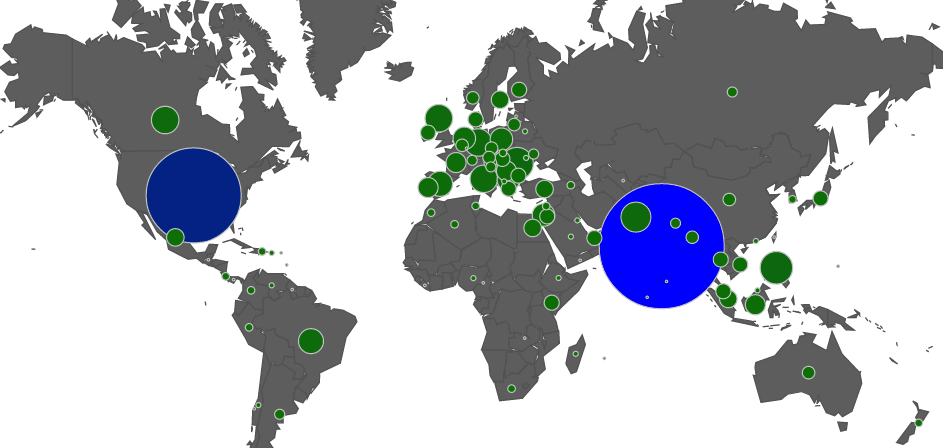
\includegraphics[width=\linewidth]{figures/turkermap-color-cropped}
\caption{The number of workers per country.  This map was generated based on geolocating the IP address of  5,284 workers in our study.  The size of the circles represents the number of workers from each country.  The two largest are India (2,022 workers) and the United States (904).  To calibrate the sizes: the Philippines has 147 workers, Egypt has 25, Russia has 10, and Sri Lanka has 4.}
\label{map}
\end{figure*}
%%%%%%%%%%%%%%%%%%%%%%%%%%%%%%%%%%%%%%%



\section{Background and Related Work}
Amazon's Mechanical Turk (MTurk) is an online marketplace for work that gives employers and researchers access to a large, low-cost, workforce. MTurk allows employers to provide micro-payments in return for workers completing micro-tasks.  The basic units of work on MTurk are called `Human Intelligence Tasks' (HITs).  MTurk was designed to accommodate tasks that are difficult for computers, but simple for people. This facilitates research into human computation, where people can be treated as a function call \cite{vonAhnThesis,Little2009,quinn-bederson:2011}.  It has application to research areas like human-computer interaction \cite{bigham-et-al:2010,bernstein-et-al:2010}, computer vision  \cite{sorkin-forsyth:2008,deng-et-al:2010,rashtchian:10}, speech processing \cite{marge:10,lane-EtAl:2010:MTURK,Parent-Eskenazi:2011,Eskenazi:2013:crowdsourcing-speech-book},  and natural language processing \cite{Snow2008,callisonburch-dredze:2010:MTURK,laws-scheible-schutze:2011:EMNLP}. 

\nocite{novotney-callisonburch:2010:NAACLHLT}

On MTurk, researchers who need work completed are called `Requesters', and workers are often referred to as `Turkers'.  MTurk is a true market, meaning that Turkers are free to choose to complete the HITs which interest them, and Requesters can price their tasks competitively to try to attract workers and have their tasks done quickly \cite{faridani-et-al:2011,singer-mittal:2011}. Turkers remain anonymous to Requesters, and all payment occurs through Amazon. Requesters are able to accept submitted work or reject work that they does not meet their standards.  Turkers are only paid if a Requester accepts their work. 

Several reports examine Mechanical Turk as an economic market \cite{ipeirotis:2010:marketplace,lehdonvirta-ernkvist:2011}.  When Amazon introduced MTurk, it first offered payment only in Amazon credits, and later offered direct payment in US dollars. More recently, it has expanded to include one foreign currency, the Indian rupee. Despite its payments being limited to two currencies or Amazon credits, MTurk claims over half a million workers from 190 countries \cite{AmazonRequesterTour}.  This suggests that its worker population should represent a diverse set of languages.

A demographic study by \newcite{ipeirotis:2010:demographics} focused on age, gender, martial status, income levels, motivation for working on MTurk, and whether workers used it as a primary or supplemental form of income.  The study contrasted Indian and US workers. \newcite{Ross2010} completed a longitudinal follow-on study. 
A number of other studies have informally investigated Turkers' language abilities.  \newcite{munro-tily:2011} compiled survey responses of 2,000 Turkers, revealing that four of the six most represented languages come from India (the top six being Hindi, Malayalam, Tamil, Spanish, French, and Telugu).  \newcite{irvine:10} had Turkers evaluate the accuracy of translations that had been automatically inducted from monolingual texts.  They examined translations of 100 words in 42 low-resource languages, and reported geolocated countries for their workers (India, the US, Romania, Pakistan, Macedonia, Latvia, Bangladesh and the Philippines).  Irvine and Klementiev discussed the difficulty of quality control and assessing the plausibility of workers' language skills for rare languages, which we address in this paper. 

Several researchers have investigated using MTurk to build parallel corpora for machine translation, a task which stands to benefit low cost, high volume  translation on demand \cite{Germann2001}.  \newcite{ambati_act} conducted a pilot study by posting 25 sentences to MTurk for Spanish, Chinese, Hindi, Telugu, Urdu, and Haitian Creole.  In a study of 2000 Urdu sentences, 
\newcite{zaidan-callisonburch:2011:ACL-HLT2011a} presented methods for achieving professional-level translation quality from Turkers by soliciting multiple English translations of each foreign sentence. 
\newcite{Zbib-etal:2012:NAACL} used crowdsourcing to construct a 1.5 million word parallel corpus of dialect Arabic and English, training a statistical machine translation system that produced higher quality translations of dialect Arabic than a system a trained on 100 times more Modern Standard Arabic-English parallel data.  \newcite{post-callisonburch-osborne:2012:WMT} used MTurk to build parallel corpora between English and six Indian languages, ranging from .5M to 1.5M words, and use them to demonstrate the efficacy of syntactic machine translation on verb-final languages.  
Several researchers have examined cost optimization using active learning techniques to select the most useful sentences or fragments to translate \cite{ambati_naacl,bloodgood-callisonburch:2010:ACL,AmbatiThesis}.

To contrast our research with previous work, the main contributions of this paper are: (1) a robust methodology for assessing the bilingual  skills of anonymous workers, (2) the largest-scale census to date of language skills of workers on MTurk, and (3) a detailed analysis of the data gathered in our study.
%, including the quality of the translations and recommendations for  languages that are feasible for near-term creation of multi-lingual technologies. 



%%%%%%%%%%%%%%% HIT UIs %%%%%%%%%%%
%\begin{figure}[h]
%\centering
%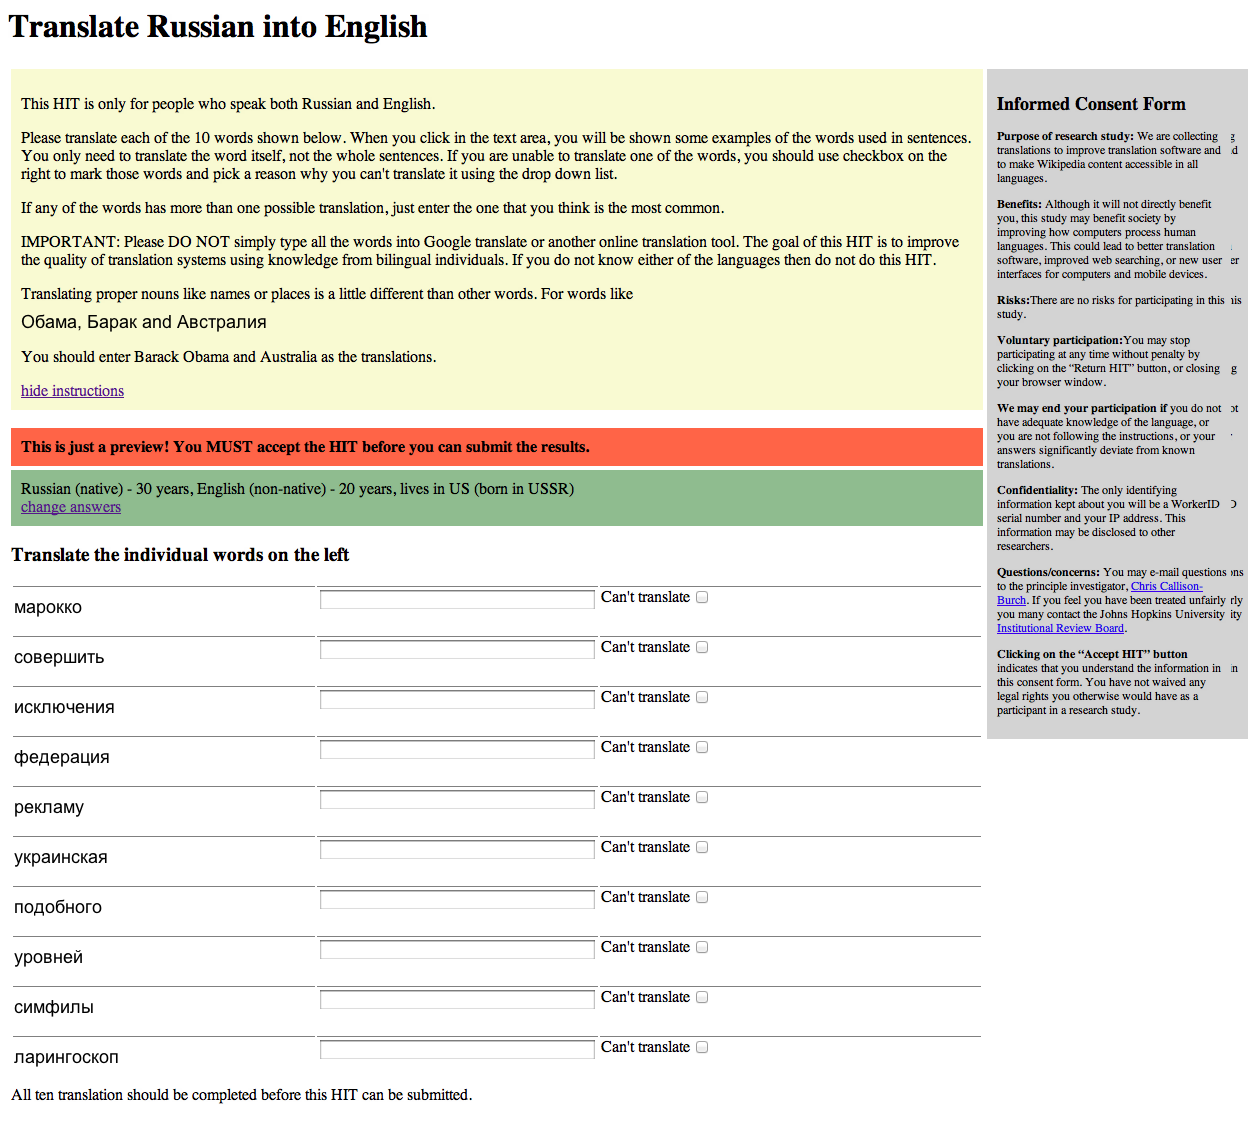
\includegraphics[width=3in]{figures/vocabulary_hit_mturk}
%\caption{Translation HIT UI}
%\label{tranhit}
%\end{figure}
%
%\begin{figure}[h]
%\centering
%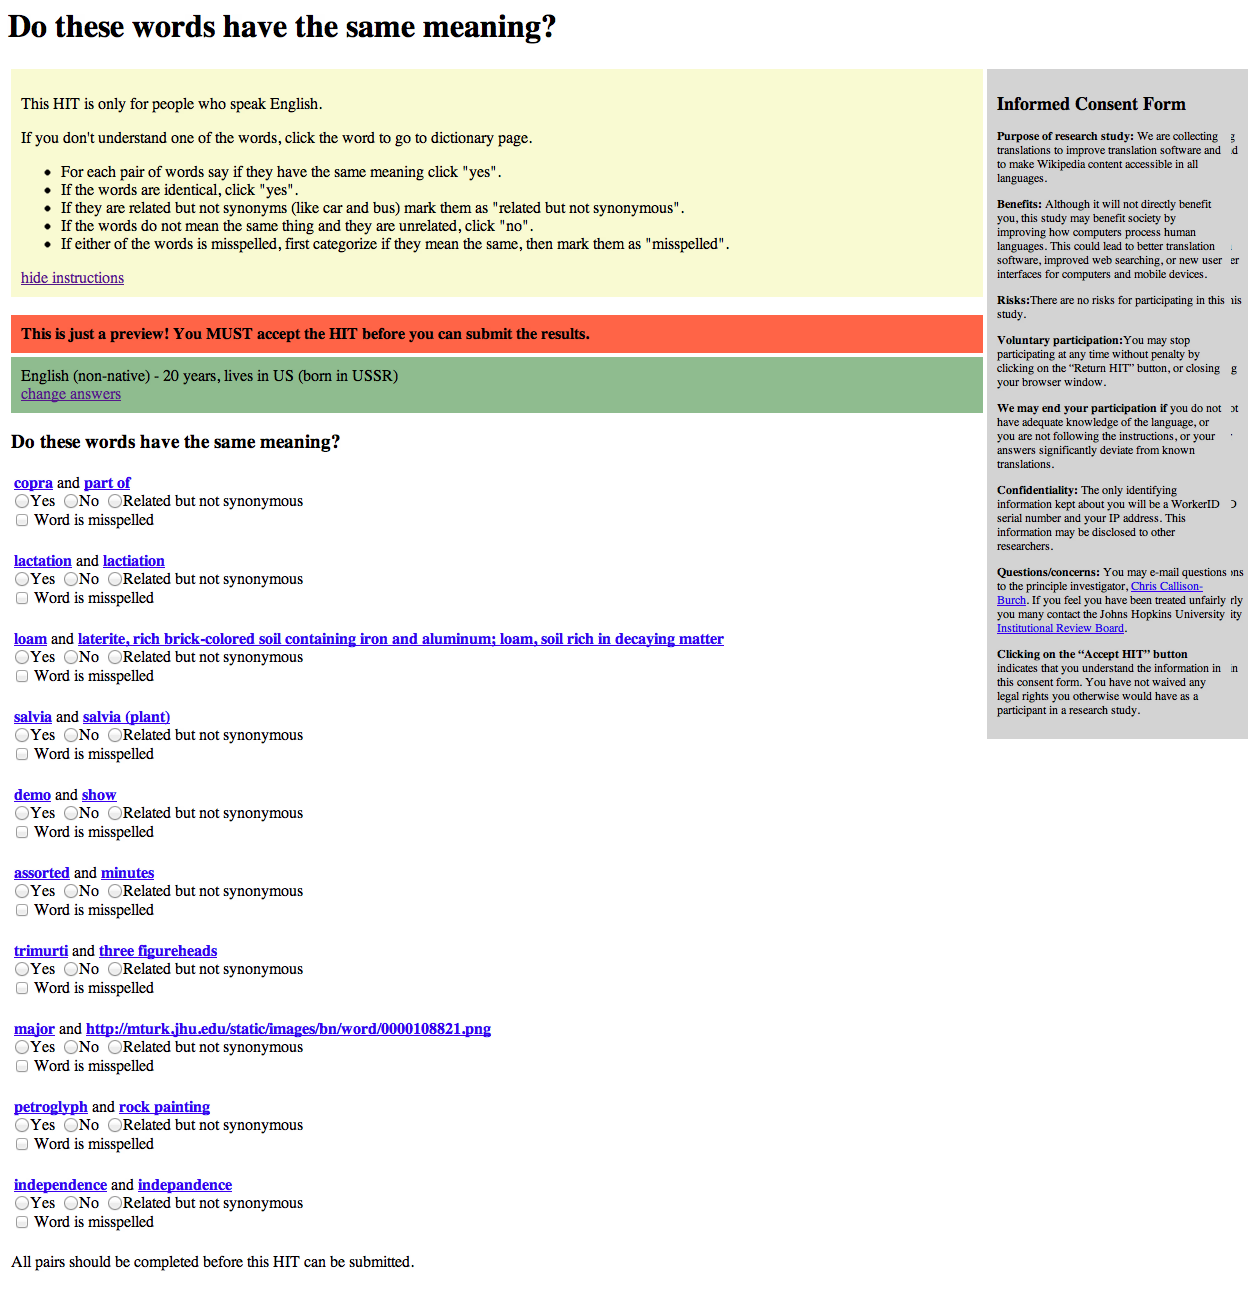
\includegraphics[width=3in]{figures/synonyms_hit_mturk}
%\caption{Evaluation HIT UI}
%\label{synhit}
%\end{figure}
%%%%%%%%%%%%%%%%%%%%%%%%%%%%%%%%%%%%%%%%%%%%%%%%%%%%%%%%

%%%%%%%%%%%%%%%% SURVEY TABLE %%%%%%%%%%%
%\begin{figure}[h]
%\begin{tabular}{lc}\hline\hline\\
%Is [HIT language/English]&\multirow{2}{*}{3,480}\\
%your native language? &\\
%How many years have you&\multirow{2}{*}{3,767}\\
%spoken [HIT language]?&\\
%How many years have you&\multirow{2}{*}{3,840}\\
%spoken English?&\\
%What country do you live in?&3,890\\
%Geolocation (collected automatically)& 5,054\\
%\hline\\
%Total workers& 5,281\\
%\hline\hline
%\end{tabular}
%\caption{Demographic survey questions and number of Turkers with valid responses for each}
%\label{survey-tab}
%\end{figure}

%\begin{table*}[h]
%\centering
%\begin{tabular}{lc}\hline\hline\\
%Is [HIT language/English] your native language? &3,480\\
%How many years have you spoken [HIT language]?&3,767\\
%How many years have you spoken English?&3,840\\
%What country do you live in?&3,890\\
%Current location (collected automatically)& 5,054\\
%\hline\\
%Total unique workers& 5,281\\
%\hline\hline
%\end{tabular}
%\caption{Demographic survey questions and number of Turkers with valid responses for each}
%\label{survey-tab}
%\end{table*}
%%%%%%%%%%%%%%%%%%%%%%%%%%%%%%%%%%%%%%%%%%%%%%%%%%%%%%%%



%%%%%%%%%%%%%%% NAT LANG PIE TABLE %%%%%%%%%%%
\begin{table}
\footnotesize
\begin{tabular}{lrlrlr}\hline\hline
%Language&\# Turkers\\
\hline
English&591&	French&63&	Vietnamese&34\\
Tamil&253&	Polish&61&	Macedonian&31\\
Malayalam&219&	Urdu&56&	Cebuano&29\\
Hindi&149&	Tagalog&54&	Swedish&26\\
Spanish&131&	Marathi&48&	Bulgarian&25\\
Telugu&87&	Russian&44&	Hungarian&23\\
Chinese&86&	Italian&43&	Swahili&23\\
Romanian&85&	Bengali&41&	Thai&22\\
Portuguese&82&	Gujarati&39&	Catalan&22\\
Arabic&74&	Hebrew&38&	Lithuanian&21\\
Kannada&72&	Dutch&37&	Punjabi&21\\
German&66&	Turkish&35&	Others &$\leq$20\\
\hline\hline
\end{tabular}
\normalsize
\caption{Self-reported native language of 3,154 bilingual Turkers. Not shown are 54 languages with $\leq$20 speakers. 
%(for a total of 423 remaining speakers).  
We omit 1,801 Turkers who did not report their native language, 243 who reported 2 native languages, and 83 who reported $\geq$3 native languages.}\label{lang-pie}
\end{table}
%%%%%%%%%%%%%%%%%%%%%%%%%%%%%%%%%%%%%%%



\section{Survey Design}
The central task in this study was to investigate Mechanical Turk's bilingual population.  We accomplished this through self-reported surveys combined with a HIT to translate individual words for over 100 languages.  We evaluate the accuracy of the workers' translations against known translations.  In cases where these were not exact matches, we used a second pass monolingual HIT, which asked English speakers to evaluate if a worker-provided translation was a synonym of the known translation.


\paragraph{Demographic questionnaire}

At the start of each HIT, Turkers were asked to complete a brief survey about their language abilities. The survey asked the following questions:
\begin{itemize}
\item Is [language] your native language? 
\item How many years have you spoken [language]? 
\item Is English your native language? 
\item How many years have you spoken English?
\item What country do you live in?
\end{itemize}
We automatically collected each worker's current location by geolocating their IP address.  A total of 5,281 unique workers completed our HITs.  Among those, 3,890 provided responses to our survey questions, and we were able to geolocate 5,054.  Figure \ref{map} plots the location of workers across 111 countries.  Table \ref{lang-pie} gives the most common self-reported native languages. 

% were not required in order to complete the HIT; survey questions and the number of valid responses received for each are listed in table \ref{survey-tab}. Although it was not required, Turkers who completed multiple HIT assignments could fill out the survey multiple times. This enabled some Turkers to report multiple native languages (see figure \ref{numlangs-tab}). While most results presented are calculated across all Turkers, figures given for distributions across native languages are calculated only from Turkers who reported a single native language.\\



\paragraph{Selection of languages}

We drew our data from the different language versions of Wikipedia.   We selected the 100 languages with the largest number of articles,\footnote{\url{http://meta.wikimedia.org/wiki/List_of_Wikipedias}} and then selected an additional 19 low resource languages with $<$10,000 articles, giving a total of 119 languages (Table \ref{wikipedia-buckets}). For each language, we chose the 1,000 most viewed articles over a 1 year period,\footnote{\url{http://dumps.wikimedia.org/other/pagecounts-raw/}} and extracted the 10,000 most frequent words from each. The resulting vocabularies served as the input to our translation HIT.

\begin{table}[h]
\scriptsize 
\begin{center}
\begin{tabular}{|p{0.95\linewidth}|}
\hline
{\sc 500k+ articles:} German (de), English (en), Spanish (es), French (fr), Italian (it), Japanese (ja), Dutch (nl), Polish (pl), Portuguese (pt), Russian (ru)\\
\hline
{\sc 100k-500k articles:} Arabic (ar), Bulgarian (bg), Catalan (ca), Czech (cs), Danish (da), Esperanto (eo), Basque (eu), Persian (fa), Finnish (fi), Hebrew (he), Hindi (hi), Croatian (hr), Hungarian (hu), Indonesian (id), Korean (ko), Lithuanian (lt), Malay (ms), Norwegian (Bokmal) (no), Romanian (ro), Slovak (sk), Slovenian (sl), Serbian (sr), Swedish (sv), Turkish (tr), Ukrainian (uk), Vietnamese (vi), Waray-Waray (war), Chinese (zh)\\
\hline
{\sc 17k-100k articles:}
Afrikaans (af), Azerbaijani (az), Belarusian (be), Bengali (bn), Bishnupriya Manipuri (bpy), Breton (br), Bosnian (bs), Cebuano (ceb), Welsh (cy), Greek (el), West Frisian (fy), Galician (gl), Gujarati (gu), Haitian (ht), Icelandic (is), Javanese (jv), Georgian (ka), Kurdish (ku), Luxembourgish (lb), Latvian (lv), Malagasy (mg), Macedonian (mk), Malayalam (ml), Marathi (mr), Low Saxon (nds), Newar / Nepal Bhasa (new), Norwegian (Nynorsk) (nn), Piedmontese (pms), Sicilian (scn), Serbo-Croatian (sh), Albanian (sq), Swahili (sw), Tamil (ta), Telugu (te), Thai (th), Tagalog (tl), Urdu (ur), Yoruba (yo)\\
\hline
{\sc $<$17k articles:} Amharic (am), Asturian (ast), Central Bicolano (bcl), Tibetan (bo), Zazaki (diq), Irish (ga), Armenian (hy), Ilokano (ilo), Kannada (kn), Neapolitan (nap), Nepali (ne), Punjabi (pa), Kapampangan (pam), Pashto (ps), Sindhi (sd), Somali (so), Sundanese (su), Uzbek (uz), Wolof (wo)\\
\hline
\end{tabular}
\end{center}
\normalsize
\caption{A list of the languages that were used in our study, grouped by the number of Wikipedia articles in the language.  Each language's code is given in parentheses.  These language codes are used in other figures throughout this paper.}\label{wikipedia-buckets}
\end{table}%

\paragraph{Translation HIT}

%Our experiments consist of two task types: a translation HIT and an evaluation HIT. 
%Examples of the interface for each are shown in figures \ref{tranhit} and \ref{synhit}.  
For the translation task, we asked Turkers to translate individual words.  We showed each word in the context of three sentences that were drawn from Wikipedia.  
Turkers were allowed to mark that they were unable to translate a word. Each task contained 10 words, 8 of which were words with unknown translations, and the other two of which were quality control words with known translations.   
We gave special instruction for translating names of people and places, giving examples of how to handle `Barack Obama' and `Australia' using their interlanguage links. For languages with non-Latin alphabets, names were transliterated. 

%
The task paid \$0.15 for the translation of 10 words.  
% 
%Assignments which had less than XXX items translated was rejected, as were workers who failed the quality control measures more than XXX\% of the time.
Each set of 10 words was independently translated by three separate workers.  5,281 workers completed 308,079 translations assignments, totaling more than 3 million words, over a period of three and a half months.

\paragraph{Gold standard translations} 
A set of gold standard translations were automatically harvested from Wikipedia  for every language to use as embedded controls. We used Wikipedia's inter-language links to pair titles of English articles with their corresponding foreign article's title.  To get a more translatable set of pairs, we excluded any pairs where: (1) the English word was not present in the WordNet ontology  \cite{miller1995wordnet}, (2) either article title was longer than a single word, (3) the English wikipedia page was a subcategory of person or place, or (4) the English and the foreign titles were identical or a substring of the other.

\paragraph{Manual evaluation of non-identical translations}
We counted all translations that exactly matched the gold standard translation as correct.  For non-exact matches we created a second-pass quality assurance HIT.  
Turkers were shown a pair of English words, one of which was a Turker's translation of the foreign word used for quality control, and the other of which was the gold-standard translation of the foreign word. Evaluators were asked whether the two words had the same meaning, and chose between three answers: `Yes', `No', or `Related but not synonymous.'  Examples of meaning equivalent pairs include: $<${\it petroglyphs, rock paintings}$>$, $<${\it demo, show}$>$ and  $<${\it loam, loam: soil rich in decaying matter}$>$.  Non-meaning equivalents included: $<${\it assorted, minutes}$>$, and $<${\it major,} URL of image$>$.  Related items were things like $<${\it sky, clouds}$>$. Misspellings like $<${\it lactation, lactiation} $>$ were judged to have same meaning, and were marked as misspelled.   3 separate Turkers judged each pair, allowing majority votes for difficult cases. 


We checked Turkers who were working on this task by embedding pairs of words which were either known to be synonyms (drawn from WordNet) or  unrelated (randomly chosen from a corpus). 
%We drew known synonyms from WordNet, and non-synonyms by pairing random words from a corpus of English (including them after they were determined to be unrelated according to WordNet).
Automating approval/rejections for the second-pass evaluation allowed the whole pipeline to be run automatically.  Caching judgments meant that we ultimately needed only 
20,955 synonym tasks to judge all of the submitted translations (a total of 55,880 unique non-matching word pairs).  These were completed by an additional 1,006 workers.  Each of these assignments included 10 word pairs and paid \$0.10.


\section{Data Analysis}

We performed an analysis of our data to address the following questions, among others:
\begin{itemize}
\item How quickly can we expect work to be completed in a particular language? 
\item What is the quality of crowdsourced translations without quality control versus with it? 
\item Do workers accurately represent their language abilities?  Should we constrain tasks by region? 
\end{itemize}


%%%%%%%%%%%%%%% COMPLETION TIME CHART %%%%%%%%%%%
\begin{figure}[h]
\centering
%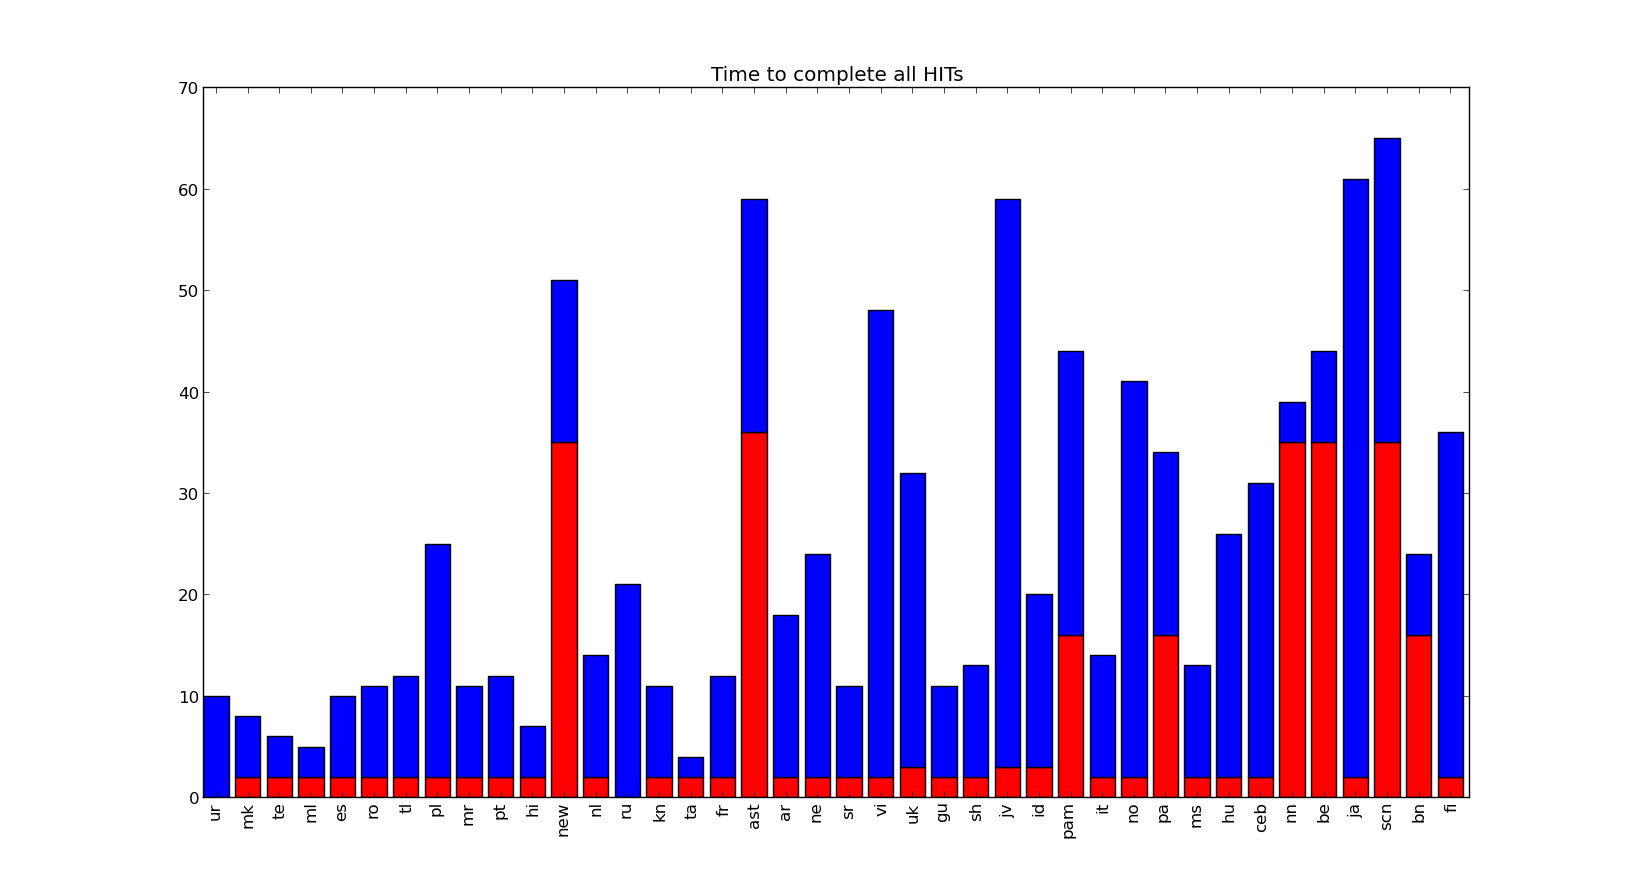
\includegraphics[height=\linewidth,angle=270]{figures/completiontime}
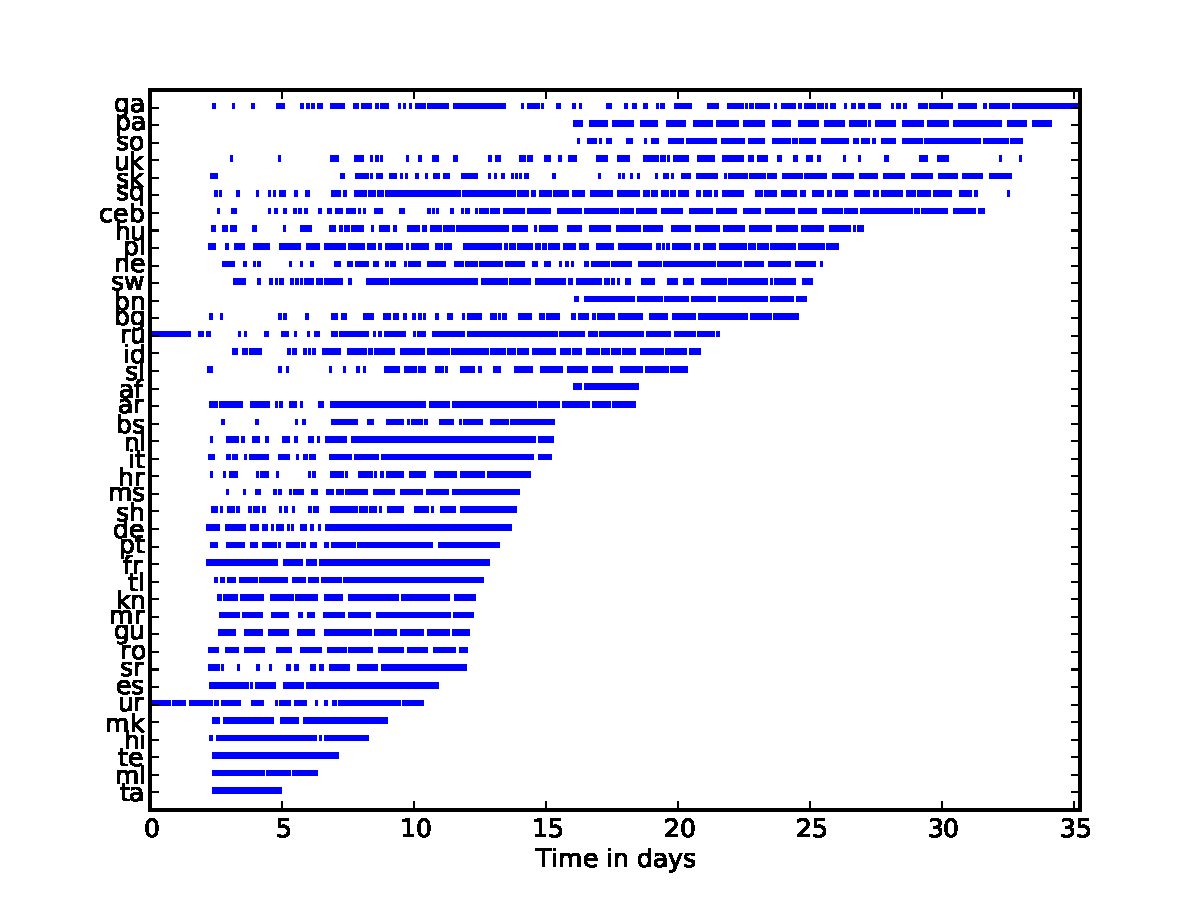
\includegraphics[height=\linewidth,angle=270]{figures/completiontime-new}
\caption{Days to complete the translation HITs for 40 of the languages. Tick marks represent the completion of individual assignments. }
\label{completion-time}
\end{figure}
%%%%%%%%%%%%%%%%%%%%%%%%%%%%%%%%%%%%%%%

\paragraph{Speed of completion}

Figure \ref{completion-time} gives the completion times for 40 languages.  
Urdu and Russian were the first languages to be launched, followed by the others 2 days later. The 10 languages to finish in the shortest amount of time were: Tamil, Malayalam, Telugu, Hindi, Macedonian, Spanish, Serbian, Romanian, Gujarati, and Marathi. 7 of the 10 fastest languages are from India, which is unsurprising given the geographic distribution of workers.  Some languages follow the pattern of having a smattering of assignments completed early, with the rate picking up later. 


\paragraph{Agreement with controls}

\paragraph{Use of machine translation}
Following \newcite{zaidan-callisonburch:2011:ACL-HLT2011a}, we rendered the words and sentences as images to reduce the ability of workers to cheat by copying-and-pasting into online MT systems.  This strategy does not prevent workers from typing the words into a MT system, if they understand the language's script.
%

%%%%%%%%%%%%%%% TURKER QUAL SUMMARY TABLE %%%%%%%%%%%
\begin{table*}
\scriptsize
%\footnotesize
\begin{center}
\begin{tabular}{lllll}
\hline\hline
&\multicolumn{2}{c}{Avg. quality (\# Turkers)}&Primary locations&Primary locations\\
&In region&Outside&of Turkers in region&of Turkers out of region\\
\hline\hline
Hindi&\textbf{0.35} (299)&0.29 (7)&India (285) UAE (5) UK (5) &Saudi Arabia (2) Russia (1) Oman (1) \\
Tamil&\textbf{0.39} (278)&0.00 (2)&India (271) US (3) Canada (2) &Tunisia (1) Egypt (1) \\
Malayalam&0.44 (235) &\textbf{0.56} (2)&India (224) UAE (6) US (3) &Saudi Arabia (1) Maldives (1) \\
Spanish&\textbf{0.71} (205)&0.60 (23)&US (131) Mexico (18) Spain (14) &India (19) Macedonia (2) New Zealand (1) \\
French&0.61 (183) &\textbf{0.80} (13)&India (68) US (48) France (25) &Greece (3) Japan (2) Netherlands (1) \\
German&\textbf{0.80} (99)&0.56 (58)&Germany (51) US (29) Austria (9) &India (47) Greece (2) UK (2) \\
Italian&\textbf{0.79} (98)&0.67 (51)&Italy (44) US (32) Romania (9) &India (38) Macedonia (2) Ireland (2) \\
Chinese&\textbf{0.22} (121)&0.18 (19)&US (79) Singapore (15) China (14) &Hongkong (6) Australia (3) Germany (2) \\
Malay&\textbf{0.76} (15)&0.72 (110)&Malaysia (8) Singapore (4) US (2) &India (106) Brunei (2) Australia (1) \\
Irish&0.61 (58) &\textbf{0.62} (59)&US (41) Ireland (13) UK (4) &India (45) Macedonia (5) Romania (5) \\
Czech&\textbf{0.70} (52)&0.62 (64)&US (19) Czech Republic (15) Serbia (5) &Macedonia (30) India (15) UK (5) \\
Turkish&\textbf{0.70} (83)&0.62 (32)&Turkey (39) US (20) Macedonia (12) &India (23) Pakistan (5) Taiwan (1) \\
Amharic&\textbf{0.17} (17)&0.02 (98)&US (14) Ethiopia (3) &India (69) Georgia (9) Macedonia (5) \\
Swedish&\textbf{0.64} (58)&0.57 (56)&US (28) Sweden (23) Finland (3) &India (26) Macedonia (10) Croatia (3) \\
Portuguese&\textbf{0.75} (107)&0.62 (4)&Brazil (46) Portugal (32) US (15) &Pakistan (1) Romania (1) Japan (1) \\
Arabic&0.21 (62) &\textbf{0.26} (48)&Egypt (19) Jordan (17) Morocco (9) &US (20) India (11) Algeria (4) \\
Kannada&\textbf{0.24} (106)&0.10 (1)&India (106) US (1) &France (1) Germany (1) \\
Russian&\textbf{0.33} (72)&0.26 (33)&US (38) Russia (8) Moldova (7) &India (17) Macedonia (4) UK (4) \\
Afrikaans&\textbf{0.73} (4)&0.64 (98)&South Africa (4) &India (93) Netherlands (2) UAE (1) \\
Sindhi&\textbf{0.16} (93)&0.11 (8)&India (55) Pakistan (37) US (1) &Macedonia (4) Georgia (2) Netherlands (1) \\
\hline\hline
\end{tabular}
\end{center}
\normalsize
\caption{The average translation quality of Turkers within a countries with larger speaker populations of a language versus Turkers from countries without large speaker populations of that language. }\label{language-regions}
\end{table*}

%%%%%%%%%%%%%%%%%%%%%%%%%%%%%%%%%%%%%%%%%%%%%%%%%%%%%%%%


\paragraph{Language skills and location}

We measured the average quality of workers who were in countries that plausibly speak a language, versus workers from countries that did not have large speaker populations of that language.  We used the Ethnologue \cite{ethnologue} to compile the list of countries where each language is spoken.  Table \ref{language-regions} compares the average translation quality of Turkers within the region of each language, and compares it to the quality of Turkers outside that region.  

Todo - overall, outliers, languages which are spoken everywhere. US workers get categorized into YY languages. 


\paragraph{Natives v. non-natives}
Todo - analyze the translation quality of natives v. non-natives.  Ideally we would plot average translation quality versus years speaking English.  Two lines: one line for native speakers of the source language, one line for non-native speakers of the target language.  We could average over all languages, and the points should show std-dev whiskers.

Other questions:
\begin{itemize}
\item Are Turkers cheating by using Google translate?  Is there a difference in their use of MT systems for Latin alphabet languages v. languages with scripts that are more difficult to type?
\item Are there flaws in our gold standard translations?  Are they too easy because they've already been indexed by Google?  Are they too hard for some languages because they are obscure scientific terms?
\item Can we select good gold standard translations for future studies?  Which translations are we confident in?
\item How well do the Turker translations match external bilingual dictionaries?  If we ranked Turkers by how well they performed on our controls, would those rankings stay stable if we ranked them based on their performance on external dictionaries? 
\item How well do Turkers agree with each other on non-control items?  Should we run a synonym HIT on all of the non-identical translations?  Would that help us understand which translations were good and which weren't?  
\end{itemize}



%%%%%%%%%%%%%%% NUM LANGUAGES TABLE %%%%%%%%%%%
%\begin{figure}[h]
%\begin{tabular}{ccc}\hline\hline
%&\# languages&\# Turkers\\ \hline
%No languages&0&1801\\
%One language&1&3154\\
%Multiple languages&2&243	\\
%&3&49\\
%&4&12\\
%&5&9\\
%&6&5\\
%&7&2\\
%&8&1\\
%&9&2\\
%&10&2\\
%&15&1\\
%\hline\hline
%\end{tabular}
%\label{numlangs-tab}
%\caption{Number of native languages reported during demographic survey.}
%\end{figure}
%%%%%%%%%%%%%%%%%%%%%%%%%%%%%%%%%%%%%%%%%%%%%%%%%%%%%%%%

%%%%%%%%%%%%%%% ASSIGNMENT SCATTER %%%%%%%%%%%
\begin{figure*}[h]
\centering
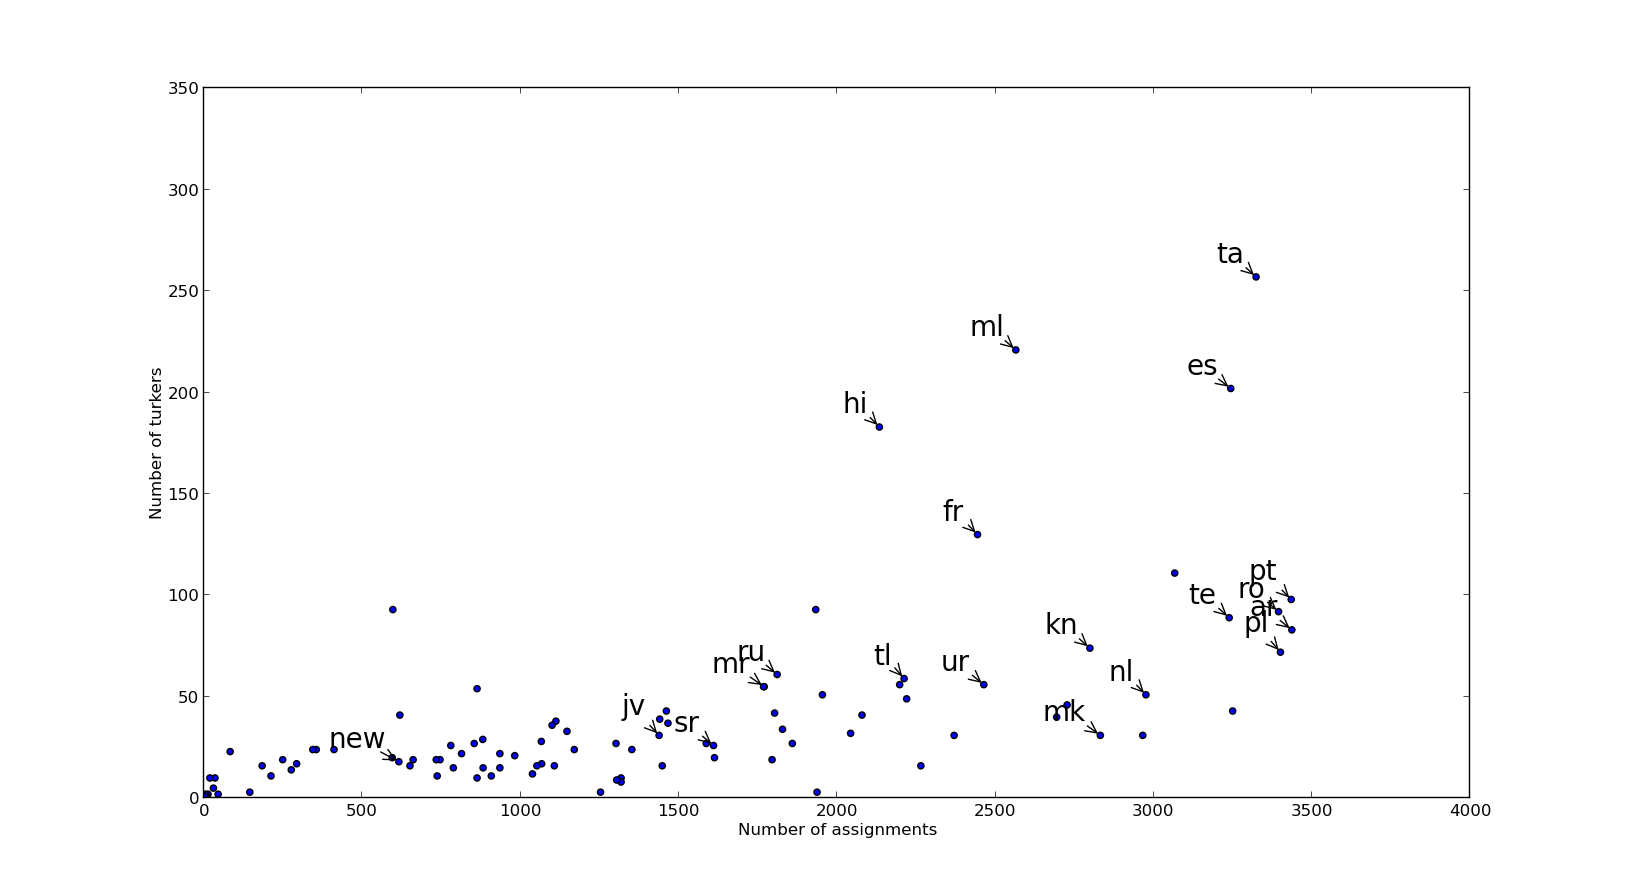
\includegraphics[width=6in]{figures/assign-turk-scatter-new}
\caption{Number of assignments and number of Turkers for each language. Each dot represents a language. Figure includes only data from Turkers who reported only one native language consistantly across assignments, representing approx. 3900 turkers across 139,000 assignments.}
\label{ass-scatter}
\end{figure*}
%%%%%%%%%%%%%%%%%%%%%%%%%%%%%%%%%%%%%%%%%%%%%%%%%%%%%%%%



Figure \ref{ass-scatter} shows the volume of HITs completed and the number of workers participating for each language. \textbf{While the bulk (22\%) of bilingual Turkers report English as their native language (see figure \ref{lang-pie}), Mechanical Turk's capacity to support the Indian languages is apparent. Hindi, Tamil, and Malayalam are especially well represented in terms of number of active translators, and Urdu, Telugu, and Macedonian are particularly productive in terms of number of assignments completed.} %As shown in figure \ref{langgeo-bar}, 11 of the top 25 languages, in terms of number of assignments submitted, were Indian languages, and the assignments for 15 of the top 25 were completed mostly or entirely by Turkers located in India. 

%%%%%%%%%%%%%%% LOCATION BAR %%%%%%%%%%%
%\begin{figure*}[h]
%\centering
%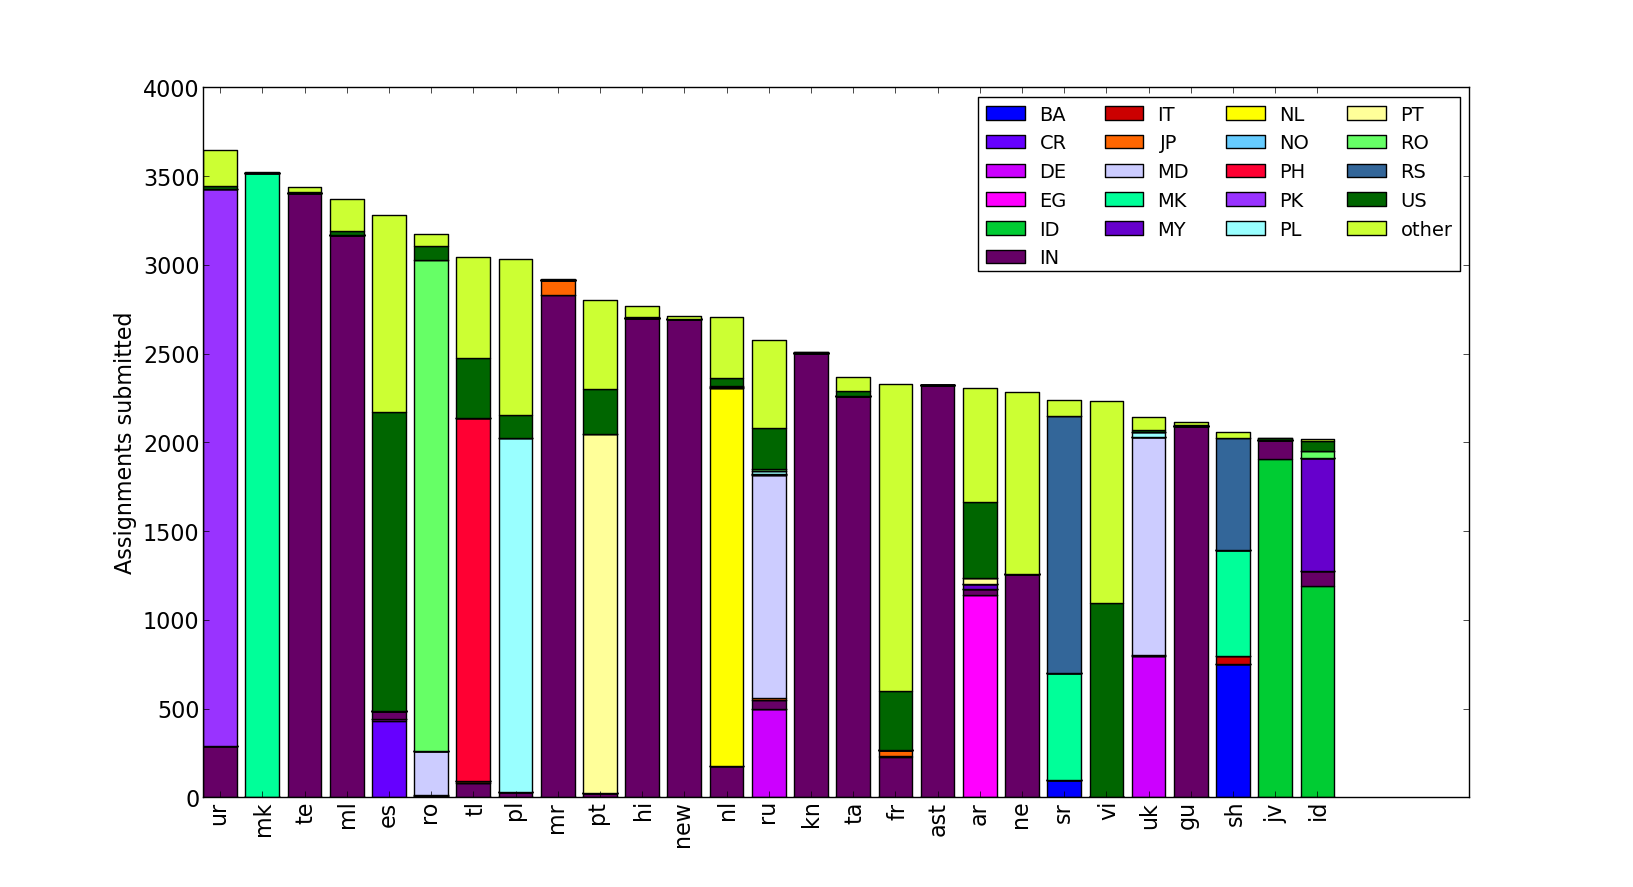
\includegraphics[width=6in]{figures/assign-langgeo-sorted}
%\caption{Geolocation of Turkers speaking 40 most represented languages, in terms of number of assignments submitted}
%\label{langgeo-bar}
%\end{figure*}
%%%%%%%%%%%%%%%%%%%%%%%%%%%%%%%%%%%%%%%%%%%%%%%%%%%%%%%%


\section{Measuring Data Quality}
%The primary challenge of using crowdsourced language data is the widely variable quality of the collected annotations. While it is possible to strengthen the signal by collecting redundant labels, this strategy becomes difficult in practice for more complex data annotation. In the case of translation, low quality translations may have a high level of agreement (for example, when many workers use google translate) while high quality, even professional translations, can be expected to vary significantly.

%In order to perform a rigorous study of translation quality, we quantify the translation quality of each Turker using our designed an internal method for quality control.  In order to address the quality of the translations we received on the dictionary task, we constructed a pipeline in which the output of the translation HIT was reviewed by humans in a second evaluation HIT, described above.  
We quantified the quality of each translation assignment based on the output of the evaluation HIT as follows: \\

\begin{align}	
	\text{Quality}(a_i) = \frac{1}{k}\sum\limits_{j=1}^{k_i}\mathbf{1}(tr_{ij} \in \texttt{syns[$g_j$]})
\end{align}	
where $a_i$ is the $i^{th}$ assignment, $k_i$ is the number of controls in $a_i$, $tr_j$ is the Turker's provided translation of control word $j$ in assignment $i$, $g_j$ is the gold standard translation of control word $j$, \texttt{syns[$g_j$]} is the set of words judged to be synonymous with $g_j$ during the second pass HIT, and $\mathbf{1}(x)$ is 1 when $x$ is true. 

Most assignments had two known words embedded, so most assignments had scores of either 0, 0.5, or 1. 

Since by-assignment quality scores are noisy and sensitive to small numbers of highly active Turkers, we report quality scores as the average per-turker quality, where a Turker's quality is just the average quality of all the assignments that the Turker completed:

\begin{align}	
	\text{Quality}(t_i) = \frac{\sum_{a_j \in \texttt{assigns[$i$]}\text{Quality}(a_j)}}{\mid \texttt{assigns[$i$]} \mid}
\end{align}	
where $t_i$ is the $i^{th}$ turker, \texttt{assigns[$i$]} is the assignments completed by turker $i$, and Quality($a$) is as above.
	
Quality for a language is then given by
\begin{align}	
	\text{Quality}(l_i) = \frac{\sum_{t_j \in \texttt{turkers[$i$]}\text{Quality}(t_j)}}{\mid \texttt{turkers[$i$]} \mid}
\end{align}	
where $l_i$ is the ith language, \texttt{turkers[$i$]} is the set of turkers who completed assignments for language $i$, and Quality($t$) is as above.




%%%%%%%%%%%%%%% MISREPORT TABLE %%%%%%%%%%%
%\begin{figure}[h]
%\centering
%\begin{tabular}{cccc}\hline\hline\\
%&Avg. & 99\%&\\
%&Quality & Conf. Int.&n\\
%Misreport&0.252&(0.244, 0.260)&10,479\\
%Correct&0.282&(0.280, 0.283)&296,911\\
%Overall&0.281&(0.279, 0.282)&307,390\\
%\hline\hline
%\end{tabular}
%\label{mism-tab}
%\caption{Quality of translations recieved from truthful versus misreporting Turkers.}
%\end{figure}
%%%%%%%%%%%%%%%%%%%%%%%%%%%%%%%%%%%%%%%%%%%%%%%%%%%%%%%%

%%%%%%%%%%%%%%% HITLANG QUALITY BAR %%%%%%%%%%%
\begin{figure*}[h]
\centering
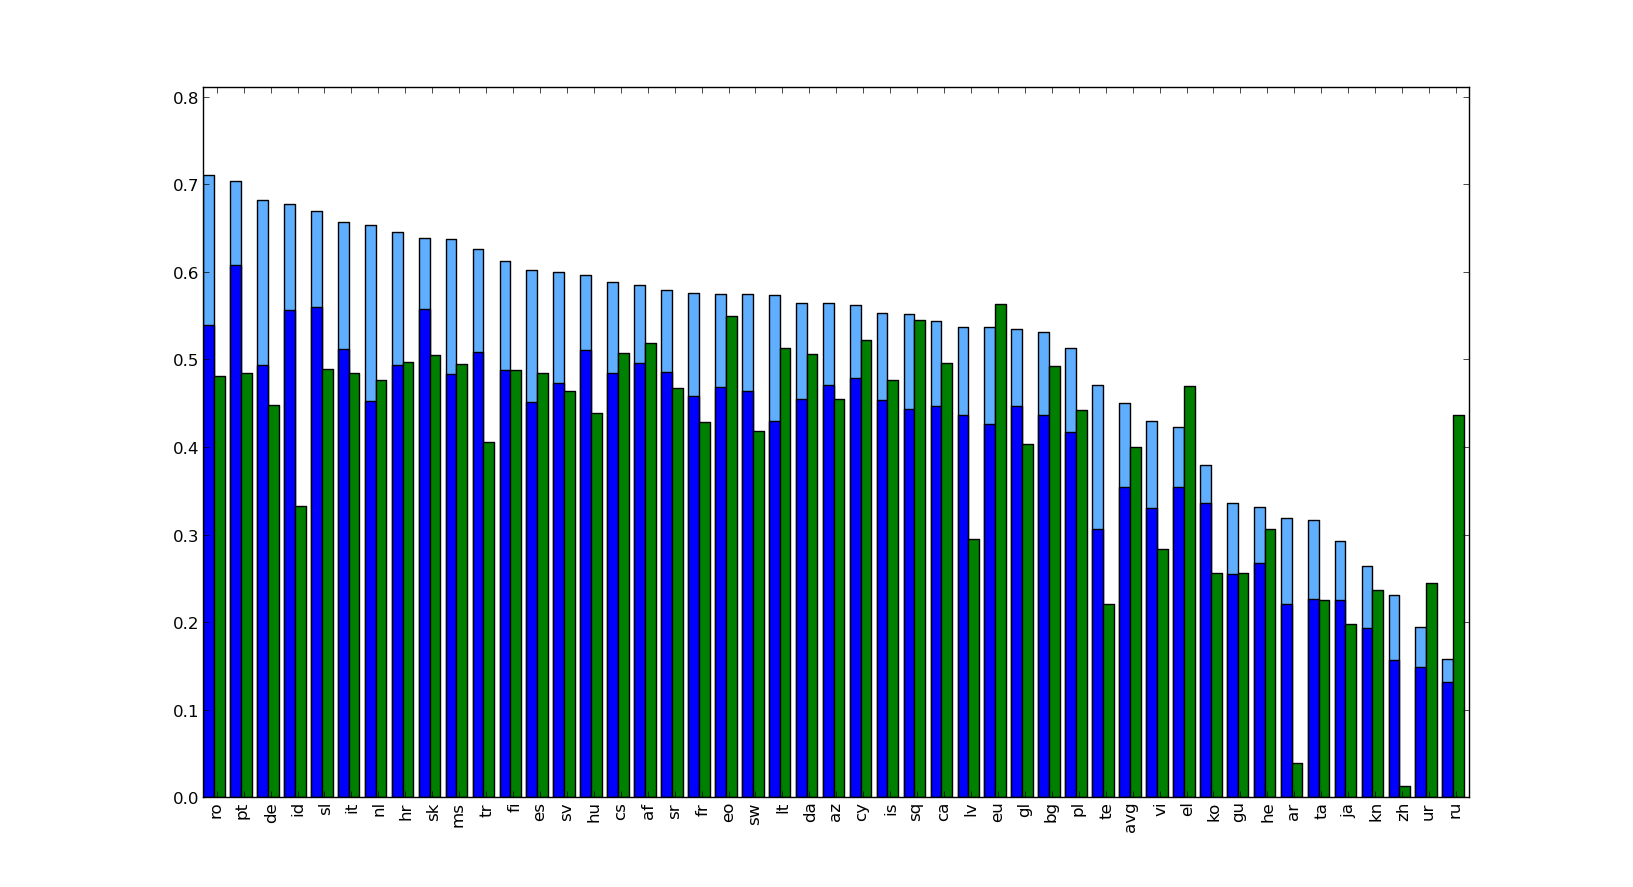
\includegraphics[width=6in]{figures/quality-hitlang-goog}
\caption{Translation quality of by source language. Blue bars show quality estimates by language and green bars show proportion of translations which matched Google Translate. Total quality is calculated as the average number of control words which were correct translations of the source word, where ”correct” means that the provided translation was judged to be synonymous with the known translation by workers in a second-
pass HIT. Dark blue bars indicate the proportion of translations which exactly matched known translations, and light blue indicate translations which were judged to be correct synonyms. Quality estimates are only show for languages with at least 50 active turkers.}
\label{hitlangqual-bar}
\end{figure*}
%%%%%%%%%%%%%%%%%%%%%%%%%%%%%%%%%%%%%%%%%%%%%%%%%%%%%%%%

Measured in this way, the average quality score across all HITs was just under 0.5. In general, countries which produced more translations did not produce lower quality translations, with India, Macedonia, and the US falling very close to average quality (figure \ref{quality-scatter}). In fact, likely as a result of the large number of India-based Turkers, most of the Indian languages fall above average quality, including Hindi, Telugu, Malayalam, Marathis, Tamil, Gujarati, Kannada, Bengali, and Punjabi, shown in figure \ref{hitlangqual-bar}. The notable exception is Urdu, which produced below average translations, likely due to the relatively low number of unique translators, making quality more susceptible to individual careless workers (see figure \ref{ass-scatter}). 


%%%%%%%%%%%%%%% NATIVE LANGUAGE QUALITY BAR %%%%%%%%%%%
%\begin{figure*}[h]
%\centering
%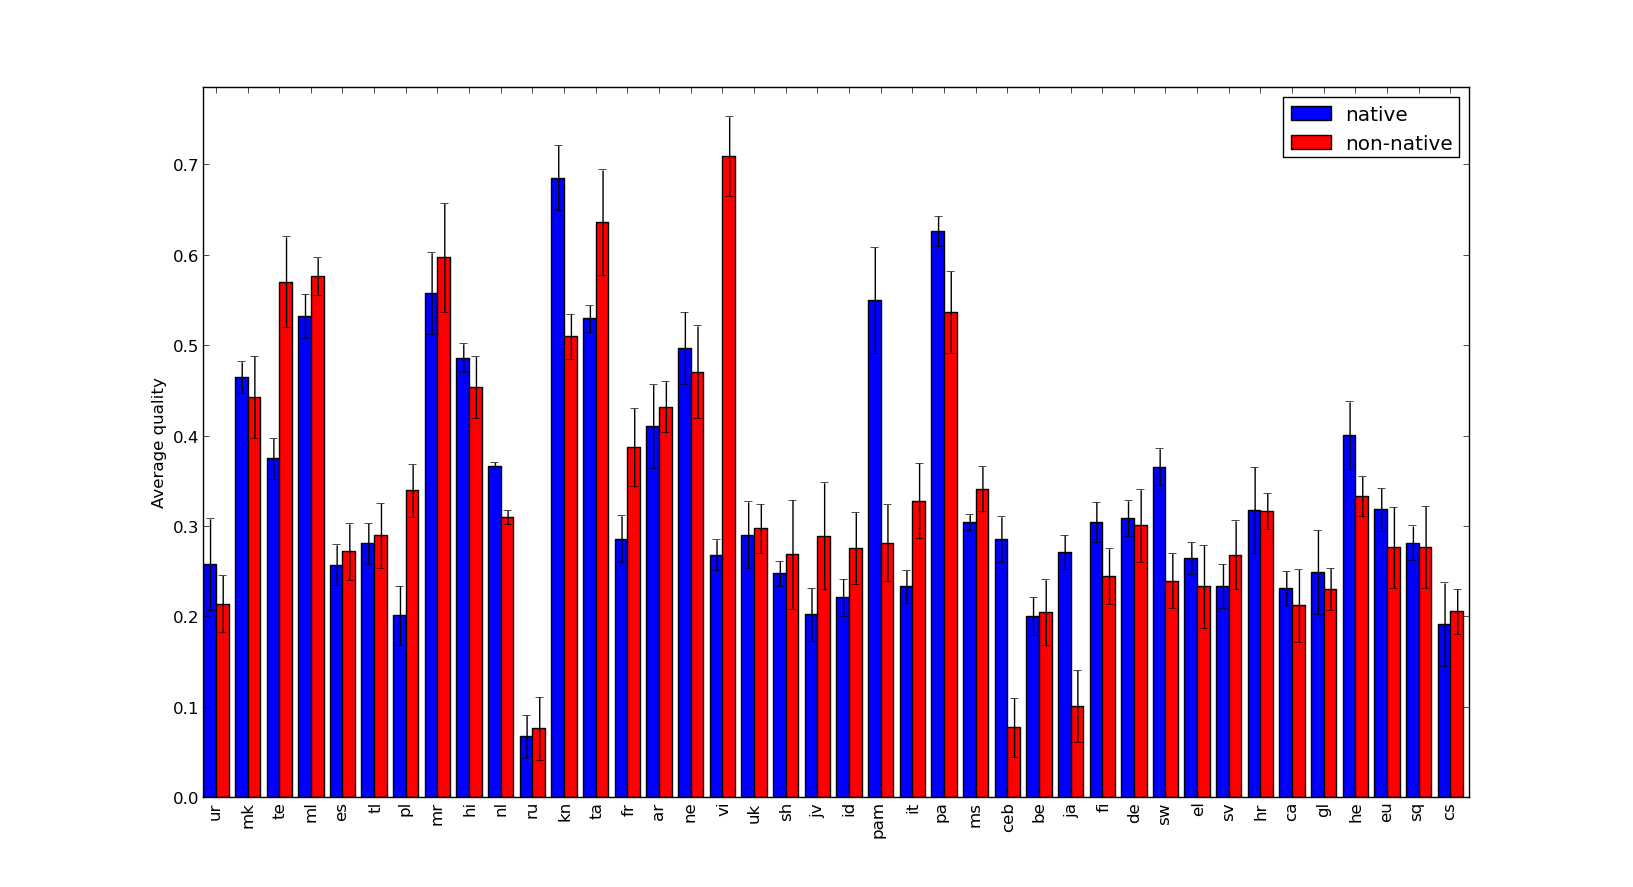
\includegraphics[width=6in]{figures/quality-natlang-sorted}
%\caption{Translation quality of native and non-native speakers}
%\label{natlangqual-bar}
%\end{figure*}
%%%%%%%%%%%%%%%%%%%%%%%%%%%%%%%%%%%%%%%%%%%%%%%%%%%%%%%%

Interestingly, native speakers do not consistently outperform non-native speakers (see figure \ref{natlangqual-bar}). In certain unique cases, such as Vietnam, non-native speakers produce significantly better translations than native speakers, possibly due to a large population of fluent US-based workers (figure \ref{langgeo-bar}). In general, the quality difference between native and non-native speakers is not significant.	


%%%%%%%%%%%%%%% QUALITY / NUM ASSIGN SCATTER %%%%%%%%%%%
\begin{figure*}[h]
\centering
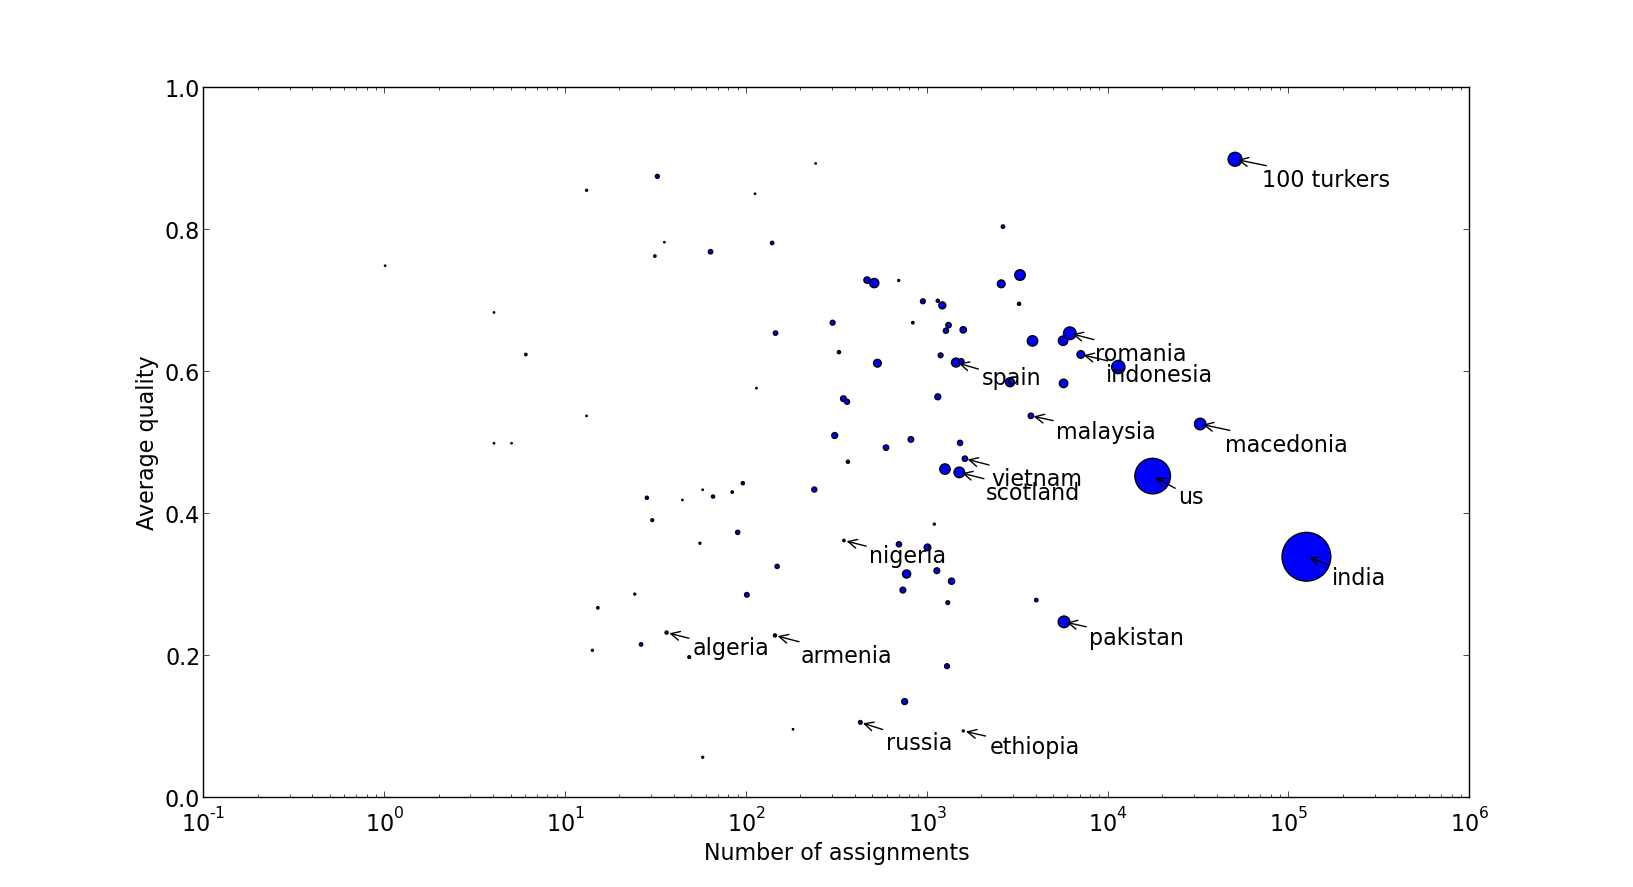
\includegraphics[width=6in]{figures/quality-scatter}
\caption{Estimated quality of translations by country. Each circle is a country, sized proportional to the number of active Turkers from that country. Quality is calculated as the average number of control words which were correct translations of the source word, where ”correct” means that the provided translation was judged to be synonymous with the known translation by workers in a second-pass HIT. Figure represents data from approx. 281,000 assignments for which geolocation was known.}
\label{quality-scatter}
\end{figure*}
%%%%%%%%%%%%%%%%%%%%%%%%%%%%%%%%%%%%%%%%%%%%%%%%%%%%%%%%

Self-reported country information is typically reliable; about 96\% of self-reported locations agreed with automatically reported locations, 
Three quarters of Turkers who reported their native language reported a single native language consistantly across all assignments (table \ref{numlangs-tab}), and of those reporting multiple native languages, the majority listed English in addition to the HIT's source language, meaning less than 5\% of Turkers gave unreasonable responses.  

\section{Discussion}
MTurk has a strong and diverse presence of bilingual workers, making it a promising resource for researchers and developers of multilingual systems. Although unfiltered data can contain large amounts of noise, crowdsourced pipelines, which contain human oversight as a means of evaluation, offer a feasible way of ensuring high quality data, even on tasks which require more complex labels. While MTurk does offer the ability to restrict workers based on country, embedded per-task controls which are checked either automatically when possible, or manually in a second-pass HIT, are likely to provide higher quality data than naive demographic filters. 

Although our research targeted bilingual workers on Mechanical Turk, and neglected monolingual workers, we believe our results reliably represent the current speaker populations, since the vast majority of the work available on the crowdsourced platform is currently English-only.  We therefore assume the number of non-English speakers is small.  In the future, it may be desirable to recruit monolingual foreign workers.  In such cases, we recommend other tests to validate their language abilities in place of our translation test.  These could include performing narrative cloze, or listening to audio files containing speech in different language and identifying their language. 


\bibliographystyle{acl2012}
\bibliography{mturk}

\end{document}
